
%% bare_conf.tex
%% V1.3
%% 2007/01/11
%% by Michael Shell
%% See:
%% http://www.michaelshell.org/
%% for current contact information.
%%
%% This is a skeleton file demonstrating the use of IEEEtran.cls
%% (requires IEEEtran.cls version 1.7 or later) with an IEEE conference paper.
%%
%% Support sites:
%% http://www.michaelshell.org/tex/ieeetran/
%% http://www.ctan.org/tex-archive/macros/latex/contrib/IEEEtran/
%% and
%% http://www.ieee.org/

%%*************************************************************************
%% Legal Notice:
%% This code is offered as-is without any warranty either expressed or
%% implied; without even the implied warranty of MERCHANTABILITY or
%% FITNESS FOR A PARTICULAR PURPOSE! 
%% User assumes all risk.
%% In no event shall IEEE or any contributor to this code be liable for
%% any damages or losses, including, but not limited to, incidental,
%% consequential, or any other damages, resulting from the use or misuse
%% of any information contained here.
%%
%% All comments are the opinions of their respective authors and are not
%% necessarily endorsed by the IEEE.
%%
%% This work is distributed under the LaTeX Project Public License (LPPL)
%% ( http://www.latex-project.org/ ) version 1.3, and may be freely used,
%% distributed and modified. A copy of the LPPL, version 1.3, is included
%% in the base LaTeX documentation of all distributions of LaTeX released
%% 2003/12/01 or later.
%% Retain all contribution notices and credits.
%% ** Modified files should be clearly indicated as such, including  **
%% ** renaming them and changing author support contact information. **
%%
%% File list of work: IEEEtran.cls, IEEEtran_HOWTO.pdf, bare_adv.tex,
%%                    bare_conf.tex, bare_jrnl.tex, bare_jrnl_compsoc.tex
%%*************************************************************************

% *** Authors should verify (and, if needed, correct) their LaTeX system  ***
% *** with the testflow diagnostic prior to trusting their LaTeX platform ***
% *** with production work. IEEE's font choices can trigger bugs that do  ***
% *** not appear when using other class files.                            ***
% The testflow support page is at:
% http://www.michaelshell.org/tex/testflow/



% Note that the a4paper option is mainly intended so that authors in
% countries using A4 can easily print to A4 and see how their papers will
% look in print - the typesetting of the document will not typically be
% affected with changes in paper size (but the bottom and side margins will).
% Use the testflow package mentioned above to verify correct handling of
% both paper sizes by the user's LaTeX system.
%
% Also note that the "draftcls" or "draftclsnofoot", not "draft", option
% should be used if it is desired that the figures are to be displayed in
% draft mode.
%
\documentclass[conference]{IEEEtran}
\usepackage{blindtext, graphicx}
\usepackage{xcolor}
\usepackage{colortbl}
% Add the compsoc option for Computer Society conferences.
%
% If IEEEtran.cls has not been installed into the LaTeX system files,
% manually specify the path to it like:
% \documentclass[conference]{../sty/IEEEtran}





% Some very useful LaTeX packages include:
% (uncomment the ones you want to load)


% *** MISC UTILITY PACKAGES ***
%
%\usepackage{ifpdf}
% Heiko Oberdiek's ifpdf.sty is very useful if you need conditional
% compilation based on whether the output is pdf or dvi.
% usage:
% \ifpdf
%   % pdf code
% \else
%   % dvi code
% \fi
% The latest version of ifpdf.sty can be obtained from:
% http://www.ctan.org/tex-archive/macros/latex/contrib/oberdiek/
% Also, note that IEEEtran.cls V1.7 and later provides a builtin
% \ifCLASSINFOpdf conditional that works the same way.
% When switching from latex to pdflatex and vice-versa, the compiler may
% have to be run twice to clear warning/error messages.






% *** CITATION PACKAGES ***
%
%\usepackage{cite}
% cite.sty was written by Donald Arseneau
% V1.6 and later of IEEEtran pre-defines the format of the cite.sty package
% \cite{} output to follow that of IEEE. Loading the cite package will
% result in citation numbers being automatically sorted and properly
% "compressed/ranged". e.g., [1], [9], [2], [7], [5], [6] without using
% cite.sty will become [1], [2], [5]--[7], [9] using cite.sty. cite.sty's
% \cite will automatically add leading space, if needed. Use cite.sty's
% noadjust option (cite.sty V3.8 and later) if you want to turn this off.
% cite.sty is already installed on most LaTeX systems. Be sure and use
% version 4.0 (2003-05-27) and later if using hyperref.sty. cite.sty does
% not currently provide for hyperlinked citations.
% The latest version can be obtained at:
% http://www.ctan.org/tex-archive/macros/latex/contrib/cite/
% The documentation is contained in the cite.sty file itself.






% *** GRAPHICS RELATED PACKAGES ***
%
\ifCLASSINFOpdf
  % \usepackage[pdftex]{graphicx}
  % declare the path(s) where your graphic files are
  % \graphicspath{{../pdf/}{../jpeg/}}
  % and their extensions so you won't have to specify these with
  % every instance of \includegraphics
  % \DeclareGraphicsExtensions{.pdf,.jpeg,.png}
\else
  % or other class option (dvipsone, dvipdf, if not using dvips). graphicx
  % will default to the driver specified in the system graphics.cfg if no
  % driver is specified.
  % \usepackage[dvips]{graphicx}
  % declare the path(s) where your graphic files are
  % \graphicspath{{../eps/}}
  % and their extensions so you won't have to specify these with
  % every instance of \includegraphics
  % \DeclareGraphicsExtensions{.eps}
\fi
% graphicx was written by David Carlisle and Sebastian Rahtz. It is
% required if you want graphics, photos, etc. graphicx.sty is already
% installed on most LaTeX systems. The latest version and documentation can
% be obtained at: 
% http://www.ctan.org/tex-archive/macros/latex/required/graphics/
% Another good source of documentation is "Using Imported Graphics in
% LaTeX2e" by Keith Reckdahl which can be found as epslatex.ps or
% epslatex.pdf at: http://www.ctan.org/tex-archive/info/
%
% latex, and pdflatex in dvi mode, support graphics in encapsulated
% postscript (.eps) format. pdflatex in pdf mode supports graphics
% in .pdf, .jpeg, .png and .mps (metapost) formats. Users should ensure
% that all non-photo figures use a vector format (.eps, .pdf, .mps) and
% not a bitmapped formats (.jpeg, .png). IEEE frowns on bitmapped formats
% which can result in "jaggedy"/blurry rendering of lines and letters as
% well as large increases in file sizes.
%
% You can find documentation about the pdfTeX application at:
% http://www.tug.org/applications/pdftex





% *** MATH PACKAGES ***
%
%\usepackage[cmex10]{amsmath}
% A popular package from the American Mathematical Society that provides
% many useful and powerful commands for dealing with mathematics. If using
% it, be sure to load this package with the cmex10 option to ensure that
% only type 1 fonts will utilized at all point sizes. Without this option,
% it is possible that some math symbols, particularly those within
% footnotes, will be rendered in bitmap form which will result in a
% document that can not be IEEE Xplore compliant!
%
% Also, note that the amsmath package sets \interdisplaylinepenalty to 10000
% thus preventing page breaks from occurring within multiline equations. Use:
%\interdisplaylinepenalty=2500
% after loading amsmath to restore such page breaks as IEEEtran.cls normally
% does. amsmath.sty is already installed on most LaTeX systems. The latest
% version and documentation can be obtained at:
% http://www.ctan.org/tex-archive/macros/latex/required/amslatex/math/





% *** SPECIALIZED LIST PACKAGES ***
%
%\usepackage{algorithmic}
% algorithmic.sty was written by Peter Williams and Rogerio Brito.
% This package provides an algorithmic environment fo describing algorithms.
% You can use the algorithmic environment in-text or within a figure
% environment to provide for a floating algorithm. Do NOT use the algorithm
% floating environment provided by algorithm.sty (by the same authors) or
% algorithm2e.sty (by Christophe Fiorio) as IEEE does not use dedicated
% algorithm float types and packages that provide these will not provide
% correct IEEE style captions. The latest version and documentation of
% algorithmic.sty can be obtained at:
% http://www.ctan.org/tex-archive/macros/latex/contrib/algorithms/
% There is also a support site at:
% http://algorithms.berlios.de/index.html
% Also of interest may be the (relatively newer and more customizable)
% algorithmicx.sty package by Szasz Janos:
% http://www.ctan.org/tex-archive/macros/latex/contrib/algorithmicx/




% *** ALIGNMENT PACKAGES ***
%
%\usepackage{array}
% Frank Mittelbach's and David Carlisle's array.sty patches and improves
% the standard LaTeX2e array and tabular environments to provide better
% appearance and additional user controls. As the default LaTeX2e table
% generation code is lacking to the point of almost being broken with
% respect to the quality of the end results, all users are strongly
% advised to use an enhanced (at the very least that provided by array.sty)
% set of table tools. array.sty is already installed on most systems. The
% latest version and documentation can be obtained at:
% http://www.ctan.org/tex-archive/macros/latex/required/tools/


%\usepackage{mdwmath}
%\usepackage{mdwtab}
% Also highly recommended is Mark Wooding's extremely powerful MDW tools,
% especially mdwmath.sty and mdwtab.sty which are used to format equations
% and tables, respectively. The MDWtools set is already installed on most
% LaTeX systems. The lastest version and documentation is available at:
% http://www.ctan.org/tex-archive/macros/latex/contrib/mdwtools/


% IEEEtran contains the IEEEeqnarray family of commands that can be used to
% generate multiline equations as well as matrices, tables, etc., of high
% quality.


%\usepackage{eqparbox}
% Also of notable interest is Scott Pakin's eqparbox package for creating
% (automatically sized) equal width boxes - aka "natural width parboxes".
% Available at:
% http://www.ctan.org/tex-archive/macros/latex/contrib/eqparbox/





% *** SUBFIGURE PACKAGES ***
%\usepackage[tight,footnotesize]{subfigure}
% subfigure.sty was written by Steven Douglas Cochran. This package makes it
% easy to put subfigures in your figures. e.g., "Figure 1a and 1b". For IEEE
% work, it is a good idea to load it with the tight package option to reduce
% the amount of white space around the subfigures. subfigure.sty is already
% installed on most LaTeX systems. The latest version and documentation can
% be obtained at:
% http://www.ctan.org/tex-archive/obsolete/macros/latex/contrib/subfigure/
% subfigure.sty has been superceeded by subfig.sty.



%\usepackage[caption=false]{caption}
%\usepackage[font=footnotesize]{subfig}
% subfig.sty, also written by Steven Douglas Cochran, is the modern
% replacement for subfigure.sty. However, subfig.sty requires and
% automatically loads Axel Sommerfeldt's caption.sty which will override
% IEEEtran.cls handling of captions and this will result in nonIEEE style
% figure/table captions. To prevent this problem, be sure and preload
% caption.sty with its "caption=false" package option. This is will preserve
% IEEEtran.cls handing of captions. Version 1.3 (2005/06/28) and later 
% (recommended due to many improvements over 1.2) of subfig.sty supports
% the caption=false option directly:
%\usepackage[caption=false,font=footnotesize]{subfig}
%
% The latest version and documentation can be obtained at:
% http://www.ctan.org/tex-archive/macros/latex/contrib/subfig/
% The latest version and documentation of caption.sty can be obtained at:
% http://www.ctan.org/tex-archive/macros/latex/contrib/caption/




% *** FLOAT PACKAGES ***
%
%\usepackage{fixltx2e}
% fixltx2e, the successor to the earlier fix2col.sty, was written by
% Frank Mittelbach and David Carlisle. This package corrects a few problems
% in the LaTeX2e kernel, the most notable of which is that in current
% LaTeX2e releases, the ordering of single and double column floats is not
% guaranteed to be preserved. Thus, an unpatched LaTeX2e can allow a
% single column figure to be placed prior to an earlier double column
% figure. The latest version and documentation can be found at:
% http://www.ctan.org/tex-archive/macros/latex/base/



%\usepackage{stfloats}
% stfloats.sty was written by Sigitas Tolusis. This package gives LaTeX2e
% the ability to do double column floats at the bottom of the page as well
% as the top. (e.g., "\begin{figure*}[!b]" is not normally possible in
% LaTeX2e). It also provides a command:
%\fnbelowfloat
% to enable the placement of footnotes below bottom floats (the standard
% LaTeX2e kernel puts them above bottom floats). This is an invasive package
% which rewrites many portions of the LaTeX2e float routines. It may not work
% with other packages that modify the LaTeX2e float routines. The latest
% version and documentation can be obtained at:
% http://www.ctan.org/tex-archive/macros/latex/contrib/sttools/
% Documentation is contained in the stfloats.sty comments as well as in the
% presfull.pdf file. Do not use the stfloats baselinefloat ability as IEEE
% does not allow \baselineskip to stretch. Authors submitting work to the
% IEEE should note that IEEE rarely uses double column equations and
% that authors should try to avoid such use. Do not be tempted to use the
% cuted.sty or midfloat.sty packages (also by Sigitas Tolusis) as IEEE does
% not format its papers in such ways.





% *** PDF, URL AND HYPERLINK PACKAGES ***
%
%\usepackage{url}
% url.sty was written by Donald Arseneau. It provides better support for
% handling and breaking URLs. url.sty is already installed on most LaTeX
% systems. The latest version can be obtained at:
% http://www.ctan.org/tex-archive/macros/latex/contrib/misc/
% Read the url.sty source comments for usage information. Basically,
% \url{my_url_here}.





% *** Do not adjust lengths that control margins, column widths, etc. ***
% *** Do not use packages that alter fonts (such as pslatex).         ***
% There should be no need to do such things with IEEEtran.cls V1.6 and later.
% (Unless specifically asked to do so by the journal or conference you plan
% to submit to, of course. )


% correct bad hyphenation here
\hyphenation{op-tical net-works semi-conduc-tor}


\begin{document}
%
% paper title
% can use linebreaks \\ within to get better formatting as desired
\title{Applying Path Finding 
Technique of an Black Army Ants in Changing Lane of Self Learned Autonomous
Car by using Agent Based Modeling}


% author names and affiliations
% use a multiple column layout for up to three different
% affiliations
\author{\IEEEauthorblockN{Chowdhury Mobarrat Haider }
\IEEEauthorblockA{Computer science\\and Engineering\\
University Of Liberal Arts Bangladesh\\
Dhaka, Bangladesh\\
Email: adnan.legend@gmail.com}
\and
\IEEEauthorblockN{Sohag Saha}
\IEEEauthorblockA{Computer science\\and Engineering\\
University Of Liberal Arts Bangladesh\\
Dhaka, Bangladesh\\
Email: sohag.saha.cse@ulab.edu.bd }
\and
\IEEEauthorblockN{Muhibbul Hasan and \\Shakhawat hossain}
\IEEEauthorblockA{Computer science\\and Engineering\\
University Of Liberal Arts Bangladesh\\
Dhaka, Bangladesh\\
Email:  }}

% conference papers do not typically use \thanks and this command
% is locked out in conference mode. If really needed, such as for
% the acknowledgment of grants, issue a \IEEEoverridecommandlockouts
% after \documentclass

% for over three affiliations, or if they all won't fit within the width
% of the page, use this alternative format:
% 
%\author{\IEEEauthorblockN{Michael Shell\IEEEauthorrefmark{1},
%Homer Simpson\IEEEauthorrefmark{2},
%James Kirk\IEEEauthorrefmark{3}, 
%Montgomery Scott\IEEEauthorrefmark{3} and
%Eldon Tyrell\IEEEauthorrefmark{4}}
%\IEEEauthorblockA{\IEEEauthorrefmark{1}School of Electrical and Computer Engineering\\
%Georgia Institute of Technology,
%Atlanta, Georgia 30332--0250\\ Email: see http://www.michaelshell.org/contact.html}
%\IEEEauthorblockA{\IEEEauthorrefmark{2}Twentieth Century Fox, Springfield, USA\\
%Email: homer@thesimpsons.com}
%\IEEEauthorblockA{\IEEEauthorrefmark{3}Starfleet Academy, San Francisco, California 96678-2391\\
%Telephone: (800) 555--1212, Fax: (888) 555--1212}
%\IEEEauthorblockA{\IEEEauthorrefmark{4}Tyrell Inc., 123 Replicant Street, Los Angeles, California 90210--4321}}




% use for special paper notices
%\IEEEspecialpapernotice{(Invited Paper)}




% make the title area
\maketitle


\begin{abstract}
This paper presents how an Autonomous car changes its lane and reach to its destination without any collation with other cars ,we have done this research by using net logo model, this paper research took inspiration from the Brazilian black army ants path finding technique which are naturally blind and find their path by the chemical trail which are called Pheromones ,this pheromones are created by the leader ants ,we will find out how other ants follow those pheromones trails and don't collide with each other and follow the same direction by being blind. We applied this technique with an autonomous car which follows the leader cars trail and changes its lane without any collation. Trails have been created by the sensor and GPS. Those cars will have 6 sensors to avoid Collations. We think this kind of research has not been done before .so we want to present some models with Net-logo how this technique can be done in real life situation by the path finding concept.
\end{abstract}
% IEEEtran.cls defaults to using nonbold math in the Abstract.
% This preserves the distinction between vectors and scalars. However,
% if the journal you are submitting to favors bold math in the abstract,
% then you can use LaTeX's standard command \boldmath at the very start
% of the abstract to achieve this. Many IEEE journals frown on math
% in the abstract anyway.

% Note that keywords are not normally used for peerreview papers.
\begin{IEEEkeywords}
Agent based modeling, path finding technique, rate of attraction, Finite state diagram, graph.
\end{IEEEkeywords}






% For peer review papers, you can put extra information on the cover
% page as needed:
% \ifCLASSOPTIONpeerreview
% \begin{center} \bfseries EDICS Category: 3-BBND \end{center}
% \fi
%
% For peerreview papers, this IEEEtran command inserts a page break and
% creates the second title. It will be ignored for other modes.
\IEEEpeerreviewmaketitle



\section{Introduction}
This Project is based on the nature technique of ants which can be applied to the autonomous car because those ants cannot see they follow their food or predator by following trails this is how an autonomous car will follow the trails without any collation and reach to its destination swiftly.\\
“Eciton burchellii” is a species of New World army ant in the genus Eciton. This species, one of the most extensively studied ant species, consists of expansive, organized swarm raids that give it the informal name Eciton Army Ants. The colony lives in bivouacs, which are routinely moved as the foraging paths change. The colony raids are maintained by the use of pheromones, can be 200 meters (660 ft) long, and employ up to 200,000 ants.this pheromones helps to find the raid of distract ants and it's also help to maintain the raid by following a same trials towards to food as well.\\
 Eciton burchellii is polymorphic,they are blind by nature and they doesn't have smell organ the main substance is the pheromones which helps them attracts to each other . when the 1st ants leaves the nest ,it creates a chemical chain which is pheromones and leaves it to its path so that he can get back with his food without getting lost but this pheromones also helps to the other ants to follow the path and similarly they also creates the same pheromones throughout the path . This is called a path finding technique.\\
The importance of this project is so much because the autonomous car can easily roam around without any GPS or sensors in the future by the help of this army ants technique. this path finding technique is so workable that a few more research and experiment can make a world changing technology .our scientist does only rely on technology research they doesn't follow the real life nature rules , this kind of nature rules can help us to identify the new way of technology .\\
this generation of science are accepting this kind of new technologies for the betterment of the people and the citizen,they even made rules of it so that it can move around freely and learned on his own if its developed by the AI machine learning technology.\\
A formal classification system for automated cars has been proposed by the National Highway Traffic Safety Administration:\\
Level 0: Driver has complete control of vehicle at all times.\\
Level 1: Some vehicle controls are automated, e.g. automatic braking.\\
Level 2: Two or more controls can be automated at the same time, e.g. cruise control and lane keeping.\\
Level 3: The driver can cede control in certain circumstances.\\
Level 4: Driver not expected to play any part in the driving process at all.\\ 
The world most successful software company like Google build a autonomous car in december 2016 and named it WAYMO and after few months later another car manufacture company named TOYOTA build a TOYOTA concept i car which is more advance and self learned autonomous car\\
Based on Google's own accident reports, their test cars have been involved in 14 collisions, of which human drivers were at fault 13 times. It was not until 2016 that the car's software caused a crash.\\
so from this inventions we can understand how much valuable the autonomous car is to the scientist and for the software companies even quantum scientist willing to merge together with the car manufacturer,that is how we got interest to work on autonomous car lane changing concept so that we can understand and experiment perfectly how and autonomous car and how a autonomous car will change its lane and doesn't collide with each other .\\
we will brief in our paper.  \\  


\subsection{contribution}
this paper presentation is being well organized so that scientist or other people who are interested on this topic can easily understand about our point. \\
We try to cover our experiment as much as we can ,we use agent based modeling in net logo so that we can see whether it is going to work or not in real life . our experiment works as we thought, because ABM is such kind of platform where we can experiment our project and we did it with the perfect eligible parameters, behavior ,size , world.\\
We used line graph to see the outcome of our results and we mention it in our papers. our target is to see where the autonomous changes its lane without any collation with each other and doesn't get distracted just like the path finding technique. And we also mentioned our future work in this field. Brief details of our project is in below.  \\


\section{background/literature review}
An autonomous car is a vehicle that is capable of sensing its environment and navigating without human input. Many such vehicles are being developed, but as of February 2017 automated cars permitted on public roads are not yet fully. No one has been yet tested by the path finding technique. \\
autonomous car are being treated as the most successful technology in this modern era. Because by the autonomous car concept many scientist are including some more features like brain optimization, self learned or modern delivery program on it.\\ 
There are more such topic in autonomous cars , lots of scientist is working on building in this kind of autonomous car projects.\\
Many of them are working on the circuit advancement, sensor development.  \\


\section{Model}
To initialize the whole project presentation we did modeling in Agent Based Modeling in Net logo .Thus our research was based on to see whether it changes its lane correctly or and and to see also the car configuration,so that the netlogo experiment can be applied with the worthy stuffs.so we have gone though with different experiments and result which were not so satisfactory but we have found lots of results which are so effective,we have used those experiment into our project to see the result and it shows us the perfect way which can lead us to the final output which we were looking for .   \\
so a brief description about model specification and Agent rules has been described below.  
\subsection{Model Specification}
Agents will be created by Breed, which will be same ant breed so that's no other agent behavior include in the world. One will be Leader and another one will be Followers .there will be multiple leaders and multiple followers which can be control by the button in the interface section.\\
there are six leaders the world,the six leaders were declared in the code.it can be increased for the better results.\\
The world contains Nest and Food.\\ 
Nest is positioned in the world nest-x 10 + min-pxcor position and nest-y -10 position from where ants will be created.\\
Food is positioned in the world set food-x max-pxcor – 10 position and food -y 40 positions from where ants will stop. \\
Agents will come out from the nest and wiggle around. wiggle angel can be increase o decrease by the button. and then it goes to the food and stop.
\begin{figure}[!h]
\centering
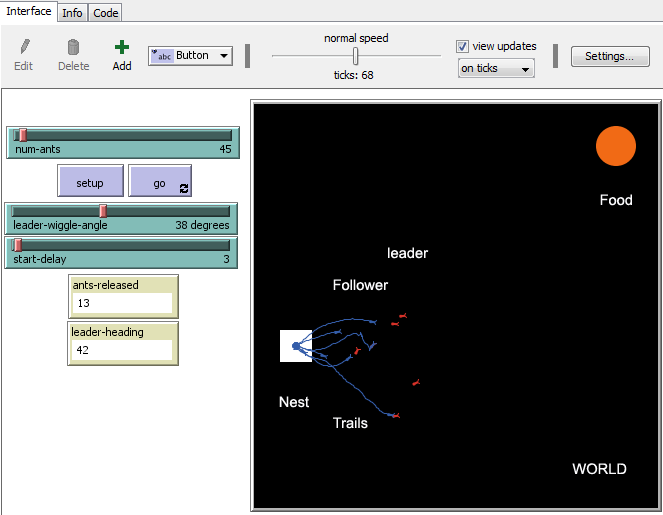
\includegraphics[scale=0.4]{Model.png}
\caption{Figure 1}
\label{fig_sim}
\end{figure}
As a leader and follower in the world. Its been shown below in Figure 1 world. Leaders are colored as RED and Followers are as blue. Leaders will lead and Followers will follow those creating Blue Pheromones Trails till they reach Food. Back end ants follow the closer line trials so that they cannot get lost from the line.
\subsection{Model Rules}
Agents will have breed of behaviors. Agents will start from Nest and stop at food.\\ 
Wiggle angle helps follower ants to move individually here and there so that others follower ants face difficult to find trails. This creates a rough trails in the world and other ants attracts, but this wiggle angle also helps to identify the distract rate of ants so that we can find it gets lost or not. Leader will follow to the food and followers will follow the leaders by creating pheromones or lane trails. Number ants can be increase or decrease by the Num Ants button. We can also decrease or increase the start time delay by other button. Which is also shown in the figure 1 .This will be the Agent behavior throughout the project. 

\section{Experiment Result}
We took line graph to see the results with individual numbers and rating of the agents so that we can find the attract and distract rate corresponding with the inter agent distance .this experiment bring us to the edge of the research so Let's take a Line graph ( figure 2) where X-axis is Num Ants and Y-axis is distance(meter) from Nest to food.\\ 
Distance from nest to food measured by Meter 0,1,2,3,4,5,6 and the population of Ants(Num Ants)was measured corresponding by the numbers.\\
Blue line in the graph  is Distance from each other Ants which is called inter agent distance.\\
Red line is Density of Ants(agents) and Green line is Distract Rate of ants from each other.\\
so when distance is 1 meter from the nest, their density and distance are same that's why their distract rate is low but when distance is high density is low their distract rate become high.\\
\begin{figure}[!h]
\centering
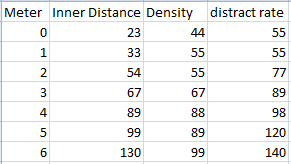
\includegraphics[scale=0.9]{Capture.png}
\caption{Numerical Range}
\label{fig_sim}
\end{figure} 

\begin{figure}[!h]
\centering
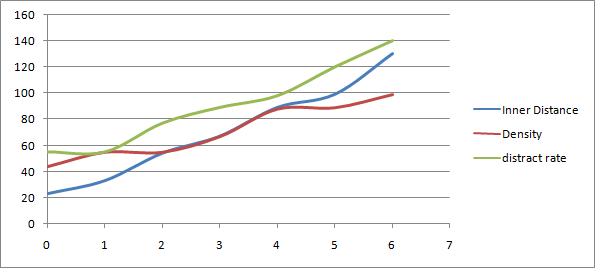
\includegraphics[scale=0.5]{graph.png}
\caption{Figure 1}
\label{fig_sim}
\end{figure}
If the inner distance range is high the distract rate will also be high.\\
here is the Numerical range and Graphical outlines of each outcomes .\\
So this experiment shows us that the high range of density has the high chance not to distract but if distance is high or too far then the rate of distract increase and it can collapse or collide with other agent .

\section{Application on Autonomous car}
Driver-less cars sense their surroundings using technology such as lidar, radar, GPS, and computer vision.\\
The sensory information is then processed to navigate appropriate pathways for the vehicle to take, avoiding any obstacles and also obeying the road signs.\\
The car uses a digital map, which can be constantly updated according to sensory input. This allows the vehicle to adapt to changing situations, as well as travel through previously unknown territories.\\
Just like a human, self-driving cars need to have sensors to understand the world around them and a brain that collects, processes and chooses specific actions based on information gathered.\\

The same goes for self-driving cars, and each autonomous vehicle is outfitted with advanced tools to gather information\\
Autonomous car have 8 sensors front ,left and right front,back,left and right back,left and right middle.\\
Including\\
1)Long range radar\\
2)Park assistance\\
3)GPS\\
4)LIDER\\
5)Sensor Camera\\
6)Artificial Intelligence based Programmed machine Learning\\

Artificial Intelligence has many applications for these vehicles; among the more immediate and obvious functions:

a) Directing the car to a gas station or recharge station when it is running low on fuel.\\
b) Adjust the trip’s directions based on known traffic conditions to find the quickest route.\\
c) Incorporate speech recognition for advanced communication with passengers.\\
d) Eye tracking for improved driver monitoring.\\
e) Natural language interfaces and virtual assistance technologies.\\

recently the world most successful software company like Google build a autonomous car in December 2016 and named it WAYMO and after few months later another car manufacture company named TOYOTA build a TOYOTA concept i car which has the YUI programmed artificial intelligence and more advance and self learned autonomous car. This is designed by following those equipment.
\begin{figure}[!t]
\centering
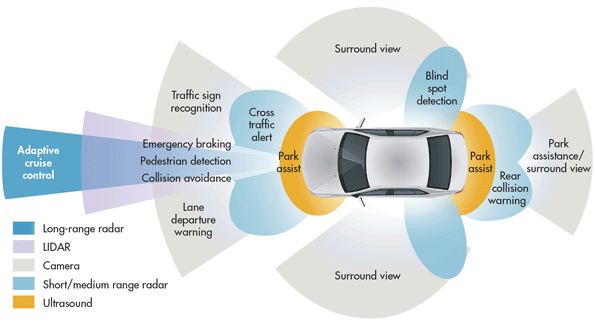
\includegraphics[scale=0.4]{car.png}
\caption{Figure 1}
\label{fig_sim}
\end{figure}
\subsection{Advantages}
a) Without the need for a driver, cars could become mini-leisure rooms. There would be more space and no need for everyone to face forwards. Entertainment technology, such as video screens, could be used to lighten long journeys without the concern of distracting the driver.\\
b) Travelers would be able to journey overnight and sleep for the duration.\\
c) Traffic could be coordinated more easily in urban areas to prevent long tailbacks at busy times. Commute times could be reduced drastically.\\
d) Reduced or non-existent fatigue from driving, plus arguments over directions and navigation would be a thing of the past.\\
e) Sensory technology could potentially perceive the environment better than human senses, seeing farther ahead, better in poor visibility, detecting smaller and more subtle obstacles, more reasons for less traffic accidents.\\
f) Speed limits could be increased to reflect the safer driving, shortening journey times.
Parking the vehicle and difficult maneuvering would be less stressful and require no special skills. The car could even just drop you off and then go and park itself.\\
g) Autonomous vehicles could bring about a massive reduction in insurance premiums for car owners.\\

h) Efficient travel also means fuel savings, cutting costs.
Reduced need for safety gaps means that road capacities for vehicles would be significantly increased.\\

i) Passengers should experience a smoother riding experience.
Self-aware cars would lead to a reduction in car theft.

\subsection{Advantages of using Pathfinding technique}
a) learning fast how to avoid collation and find the best way.\\
b) changing the lane smoothly and swiftly\\
c) changing the lane on worst case scenario like JAM , huge traffic.\\
d) self learning experience . \\
e) Decision making in every situation using AI . \\
There are some disadvantages too which should not be neglected because besides advantages we should also focus of the project disadvantages too.\\
1) Truck drivers and taxi drivers will lose their jobs, as autonomous vehicles take over.\\ 
2) Driver-less cars would likely be out of the price range of most ordinary people when generally introduced, likely costing over 100,000 dollar or more than that.\\
3) Machine Malfunction can occur real life worst case scenario.\\
4)
\section{Future Works}
Recent scientist have already created lots of autonomous cars  with advance facilities and equipment which took the usage of technology in whole new level in the science world. They included lots of feature ,these are the top most main technology equipment which they used in the autonomous car.\\
Domi is as autonomous car living room , it can have both car and living room facilitated automated system , which have the different and unique technologies including artificial intelligence on it.\\
These days, it’s easy to fall into the trap of thinking that anything really important in tech only happens in the cloud. After all, that’s where all the excitement, investment and discussion seems to be. And there are indeed innumerable efforts to not only build software for the cloud, but also to use the cloud to completely reinvent companies or even industries.\\

As important as these cloud-based developments may be, however, they shouldn’t supercede many of the equally exciting capabilities being brought to life on the edge of today’s networks. While these endpoints, or edge devices, used to be limited to smartphones, PCs and tablets, there’s now an explosion of new options for creating, manipulating, viewing, analyzing and storing data. From VR headsets to smart digital assistants to intelligent tractors, the range of edge devices is enormous and shows no signs of slowing down anytime soon.\\
we are creating more way of scope to enhance the box and think for the betterment of the people , we are still working on the concept which can show you the results of not having error or miss calculated algorithm function .\\
more country is supporting on driverless cars that is why there countries like Florida
California,Michigan,Nevada\\
In 2015, two more states are set to join the four above:
Washington D.C,Virginia\\
this brazillain black ants concepts leads us to a new concept of building a autonous which can even fly and swim under water freely without any obstacle or problems\\
“The most important thing for people to realize is that consumers are worried that autonomous driving is not safe. It will be safe,” confirms Winter.\\
At its core, Artificial Intelligence is a complex algorithm that mimics how the human brain learns. Instead of hard-coding an autonomous car with thousands of “If-Then” statements, software engineers create an algorithm that outlines to the car’s onboard computers various examples of what is right, wrong, safe, and unsafe for the car to perform.\\

This type of approach to automotive engineering may seem counter-intuitive, but in reality, artificial intelligence algorithms are the only solution to the dynamic driving conditions of public roads.\\
Self-driving cars are rapidly evolving as we see unimaginable innovation in hardware, software, and computing capabilities. However, as we progress toward advanced automobiles, one of the limiting factors restricting the growth of this field is Artificial Intelligence and machine learning.\\

Unless autonomous cars can interpret the many types of objects and situations surrounding them, they can’t make adequate decisions. Instead of developing millions of rules, a sophisticated learning algorithm needed to develop and standardized across the industry.\\


In the future car development we think our project should help to create a self optimized  autonomous car .This path finding technique of black army ants are incredible and surprising so this can make changes to the autonomous car industry we think .so that's why we are giving our project research so much importance.\\
\begin{figure}[!h]
\centering
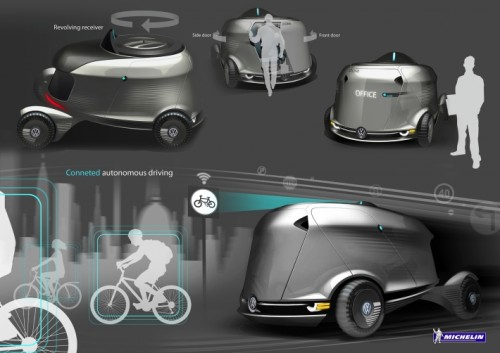
\includegraphics[scale=0.5]{domi.png}
\caption{Figure 1}
\label{fig_sim}
\end{figure}
% needed in second column of first page if using \IEEEpubid
%\IEEEpubidadjcol

% An example of a floating figure using the graphicx package.
% Note that \label must occur AFTER (or within) \caption.
% For figures, \caption should occur after the \includegraphics.
% Note that IEEEtran v1.7 and later has special internal code that
% is designed to preserve the operation of \label within \caption
% even when the captionsoff option is in effect. However, because
% of issues like this, it may be the safest practice to put all your
% \label just after \caption rather than within \caption{}.
%
% Reminder: the "draftcls" or "draftclsnofoot", not "draft", class
% option should be used if it is desired that the figures are to be
% displayed while in draft mode.
%
%\begin{figure}[!t]
%\centering
%\includegraphics[width=2.5in]{myfigure}
% where an .eps filename suffix will be assumed under latex, 
% and a .pdf suffix will be assumed for pdflatex; or what has been declared
% via \DeclareGraphicsExtensions.
%\caption{Simulation Results}
%\label{fig_sim}
%\end{figure}

% Note that IEEE typically puts floats only at the top, even when this
% results in a large percentage of a column being occupied by floats.


% An example of a double column floating figure using two subfigures.
% (The subfig.sty package must be loaded for this to work.)
% The subfigure \label commands are set within each subfloat command, the
% \label for the overall figure must come after \caption.
% \hfil must be used as a separator to get equal spacing.
% The subfigure.sty package works much the same way, except \subfigure is
% used instead of \subfloat.
%
%\begin{figure*}[!t]
%\centerline{\subfloat[Case I]\includegraphics[width=2.5in]{subfigcase1}%
%\label{fig_first_case}}
%\hfil
%\subfloat[Case II]{\includegraphics[width=2.5in]{subfigcase2}%
%\label{fig_second_case}}}
%\caption{Simulation results}
%\label{fig_sim}
%\end{figure*}
%
% Note that often IEEE papers with subfigures do not employ subfigure
% captions (using the optional argument to \subfloat), but instead will
% reference/describe all of them (a), (b), etc., within the main caption.


% An example of a floating table. Note that, for IEEE style tables, the 
% \caption command should come BEFORE the table. Table text will default to
% \footnotesize as IEEE normally uses this smaller font for tables.
% The \label must come after \caption as always.
%
%\begin{table}[!t]
%% increase table row spacing, adjust to taste
%\renewcommand{\arraystretch}{1.3}
% if using array.sty, it might be a good idea to tweak the value of
% \extrarowheight as needed to properly center the text within the cells
%\caption{An Example of a Table}
%\label{table_example}
%\centering
%% Some packages, such as MDW tools, offer better commands for making tables
%% than the plain LaTeX2e tabular which is used here.
%\begin{tabular}{|c||c|}
%\hline
%One & Two\\
%\hline
%Three & Four\\
%\hline
%\end{tabular}
%\end{table}


% Note that IEEE does not put floats in the very first column - or typically
% anywhere on the first page for that matter. Also, in-text middle ("here")
% positioning is not used. Most IEEE journals use top floats exclusively.
% Note that, LaTeX2e, unlike IEEE journals, places footnotes above bottom
% floats. This can be corrected via the \fnbelowfloat command of the
% stfloats package.



\section{Conclusion}
 By doing all that experiment in net logo with agent based modeling we came with a decision that if we apply this path finding technique in automated it could be a big success in this century. because no one has been applied this blind black army ants path finding technique in the autonomous cars .They use to run the autonomous car  by GPS and sensors cameras but not with this kind of technique .\\
Google's vehicles have traversed San Francisco's Lombard Street, famed for its steep hairpin turns, and through city traffic. The vehicles have driven over the Golden Gate Bridge and around Lake Tahoe. The system drives at the speed limit it has stored on its maps and maintains its distance from other vehicles using its system of sensors. The system provides an override that allows a human driver to take control of the car by stepping on the brake or turning the wheel, similar to cruise control systems already found in many cars today.\\
As of 28 August 2014, according to Computer World Google's self-driving cars were in fact unable to use about 99 percent of US roads. As of the same date, the latest prototype had not been tested in heavy rain or snow due to safety concerns. Because the cars rely primarily on pre-programmed route data, they do not obey temporary traffic lights and, in some situations, revert to a slower "extra cautious" mode in complex unmapped intersections. The vehicle has difficulty identifying when objects, such as trash and light debris, are harmless, causing the vehicle to veer unnecessarily. Additionally, the lidar technology cannot spot some potholes or discern when humans, such as a police officer, are signaling the car to stop. Google projects plan on having these issues fixed by 2020.\\
In January 2016, U.S. Transportation Secretary Anthony Foxx unveiled new policy that updates the National Highway Traffic Safety Administration's (NHTSA) 2013 preliminary policy statement on autonomous vehicles. This announcement was made at the North American International Auto Show in Detroit in conjunction with a commitment of nearly 4 billion dollar over the next 10 years to accelerate the development and adoption of safe vehicle automation. The new policy is designed to facilitate and encourage the development and deployment of technologies with the potential to save lives. Within six months, NHTSA will propose guidance to industry on establishing principles of safe operation for fully autonomous vehicles.\\
world is changing day by day, more people relay on the technology rather than the physical activities.This technology can be very much helpful and can be disaster either.this kind of technology ring the most of the change into the real life scenario because more software companies like Google , Apple wants to take over the car companies so that they can give their best support to brand them and can reach to the high level of the industry as well. \\
 so if we do more research and experiment in this field we think we can achieve more astonishing stuffs for the smart cities of the new world citizens .hope this paper presentation helps people to get attracted in this kind of fields and share their opinion to the world . Because world is our we need to change as we want.





% if have a single appendix:
%\appendix[Proof of the Zonklar Equations]
% or
%\appendix  % for no appendix heading
% do not use \section anymore after \appendix, only \section*
% is possibly needed

% use appendices with more than one appendix
% then use \section to start each appendix
% you must declare a \section before using any
% \subsection or using \label (\appendices by itself
% starts a section numbered zero.)
%



\section*{Acknowledgment}


On behalf of the Group Mr.Chowdhury Mobarrat Haider would like to thank to Dr. Sifat Momen sir to Helping us all the way through out the research of this Project.\\
Without him we couldn't complete our experiments and result so quickly,we will always be  to him for this kind of love and support. 


% Can use something like this to put references on a page
% by themselves when using endfloat and the captionsoff option.
\ifCLASSOPTIONcaptionsoff
  \newpage
\fi



% trigger a \newpage just before the given reference
% number - used to balance the columns on the last page
% adjust value as needed - may need to be readjusted if
% the document is modified later
%\IEEEtriggeratref{8}
% The "triggered" command can be changed if desired:
%\IEEEtriggercmd{\enlargethispage{-5in}}

% references section

% can use a bibliography generated by BibTeX as a .bbl file
% BibTeX documentation can be easily obtained at:
% http://www.ctan.org/tex-archive/biblio/bibtex/contrib/doc/
% The IEEEtran BibTeX style support page is at:
% http://www.michaelshell.org/tex/ieeetran/bibtex/
%\bibliographystyle{IEEEtran}
% argument is your BibTeX string definitions and bibliography database(s)
%\bibliography{IEEEabrv,../bib/paper}
%
% <OR> manually copy in the resultant .bbl file
% set second argument of \begin to the number of references
% (used to reserve space for the reference number labels box)
\begin{thebibliography}{1}

\bibitem{IEEEhowto:kopka}
Net logo , \emph{Agent BAsed Modelling }, 6th~ed.\hskip 1em plus
  0.5em minus 0.4em\relax 2017.
  
  \bibitem{IEEEhowto:kopka}
Net logo , \emph{Ant lines Modelling library }, 6th~ed.\hskip 1em plus
  0.5em minus 0.4em\relax 2017.
  
  \bibitem{IEEEhowto:kopka}
Net logo , \emph{Agent BAsed Modelling }, 3rd~ed.\hskip 1em plus
  0.5em minus 0.4em\relax Harlow, England: Addison-Wesley, 1999.
\bibitem{IEEEhowto:kopka}
Autonomous Car,wiki \emph{en.wikipedia.org }, 3rd~ed.\hskip 1em plus
  0.5em minus 0.4em\relax Liden, Daniel, WiseGeek. Retrieved 11 October 2013.

  \bibitem{IEEEhowto:kopka}
eciton burcelli ,wiki \emph{en.wikipedia.org }, 6th~ed.\hskip 1em plus
  0.5em minus 0.4em\relax Willson, S. K ,2011.

\bibitem{IEEEhowto:kopka}
adv and dis-adv of driverless car \emph{axleaddicts.com }, 7th~ed.\hskip 1em plus
  0.5em minus 0.4em\relax Willson, S. K ,2010.

\end{thebibliography}



% biography section
% 
% If you have an EPS/PDF photo (graphicx package needed) extra braces are
% needed around the contents of the optional argument to biography to prevent
% the LaTeX parser from getting confused when it sees the complicated
% \includegraphics command within an optional argument. (You could create
% your own custom macro containing the \includegraphics command to make things
% simpler here.)
%\begin{biography}[{\includegraphics[width=1in,height=1.25in,clip,keepaspectratio]{mshell}}]{Michael Shell}
% or if you just want to reserve a space for a photo:

\begin{IEEEbiography}[{\includegraphics[width=1in,height=1.25in,clip,keepaspectratio]{picture}}]{John Doe}
\blindtext
\end{IEEEbiography}

% You can push biographies down or up by placing
% a \vfill before or after them. The appropriate
% use of \vfill depends on what kind of text is
% on the last page and whether or not the columns
% are being equalized.

%\vfill

% Can be used to pull up biographies so that the bottom of the last one
% is flush with the other column.
%\enlargethispage{-5in}




% that's all folks
\end{document}


